
\section{Quản lí mã nguồn}
\subsection{Cấu trúc cây thư mục}
Việc cần làm đầu tiên và quan trọng nhất là tổ chức files và các thư mục. Với một thiết kế tốt thì khi làm việc chung giữa nhiều người sẽ ít bị đụng độ. Nhóm lựa chọn cách chia mỗi thành phần của trang ra từng module tách biệt với nhau, thuận lợi cho việc mở rộng và bảo trì, bảo dưỡng.

Dựa vào kiến trúc hệ thống mà nhóm đã thiết kế ở trên, nhóm đã thiết kế cấu trúc mã nguồn như sau:
\begin{center}
  \captionsetup{type=figure}
  \includegraphics[width=15cm]{document/image/cauTrucThuMuc.png}
  \captionof{figure}{Cây thư mục của hệ thống}
\end{center}
\clearpage
% Nhóm chia các chức năng vào từng module riêng, các module được thiết kế thống nhất theo mô hình MVC kết hợp với Redux. 

% Cách chia module này thuận lợi cho phân chia công việc, tránh đụng độ trong phát triển hệ thống, dễ dàng thêm các module mới trong quá trình mở rộng, giúp cho việc tìm và sửa lỗi trong quá trình bảo trì trở nên đơn giản hơn.
% \begin{figure}[H]
%     \centering
%     \begin{subfigure}[b]{0.4\linewidth}
%         \includegraphics[width=\linewidth]{image/module.png}
%         \caption{Thư mục module}
%     \end{subfigure}
%     \begin{subfigure}[b]{0.4\linewidth}
%         \includegraphics[width=\linewidth]{image/moduleDetail.png}
%         \caption{Chi tiết từng module}
%     \end{subfigure}
%     \caption{Thư mục module của hệ thống}
% \end{figure}
% \clearpage
\subsection{Git}
\begin{center}
  \captionsetup{type=figure}
  \includegraphics[width=15cm]{document/image/AAEAAQAAAAAAAAdxAAAAJDdlNTkxZDk0LTJlNmItNDc1NS1hODdiLTQwZTZiZDdmN2Y0Ng.png}
  \captionof{figure}{Git}
\end{center}

Git là hệ thống quản lý phiên bản phân tán (Distributed Version Control System).\par 
Git hỗ trợ quản lý code và các phiên bản thay đổi của kho chứa mã nguồn (repository), chúng ta có thể thay đổi mã nguồn bằng cách commit và push lên hệ thống này. Git mạnh hơn những hệ thống quản lý mã nguồn khác ở chỗ Git có hỗ trợ cho việc phân nhánh, tạo label, điều này hỗ trợ rất tốt cho việc làm teamwork, chia task cho các thành viên thành những nhánh khác nhau, tạo PR(pull request) trước khi merge vào nhánh chính.\par

\textbf{Vì sao cần sử dụng Git?}
\begin{itemize}
    \item Git dễ sử dụng, an toàn và hiệu quả.
    \item Có thể giúp làm việc nhóm hiệu quả hơn thông qua việc phân nhánh (branch).
    \item Dễ dàng hơn cho việc deployment.
    \item Có thể làm việc bất cứ đâu, bất cứ máy nào, chỉ cần clone mã nguồn hoặc một nhánh nào đó của mã nguồn để làm việc.
\end{itemize}

\subsection{Git Hub}
\begin{center}
  \captionsetup{type=figure}
  \includegraphics[width=15cm]{document/image/github.png}
  \captionof{figure}{Github}
\end{center}

Github là một dịch vụ máy chủ repository công cộng. Mỗi người có thể đăng kí tài khoản để quản lý mã nguồn (repository) riêng của mình. Github hỗ trợ tạo repository ở trạng thái công cộng (public) hoặc chỉ riêng mình người sử dụng (private).\par 
Đường dẫn mã nguồn của dự án:

\href{https://github.com/tri721305/luanvan2020}{Du Lịch Goz}
\clearpage
\section{Giao diện người dùng}
Dựa vào thiết kế UI đã thiết kế nhóm đã tiến hành hiện thực giao hiện người dùng như sau: 
\subsection{Giao diện trang chủ}
\begin{center}
  \includegraphics[width=15cm]{document/image/Home1.png}
\end{center}
\begin{center}
  \includegraphics[width=15cm]{document/image/Home2.png}
\end{center}
\clearpage
\begin{center}
  \captionsetup{type=figure}
  \includegraphics[width=15cm]{document/image/home5.png}
  \captionof{figure}{Trang chủ}
\end{center}


\subsection{Giao diện đăng nhập}
\begin{center}
  \captionsetup{type=figure}
  \includegraphics[width=15cm]{document/image/loginPage.png}
  \captionof{figure}{Trang đăng nhập}
\end{center}

\subsection{Giao diện danh sách bài Review}
\begin{center}
    \includegraphics[width=15cm]{document/image/dsBaiReview.png}
\end{center}
\clearpage
\begin{center}
  \captionsetup{type=figure}
  \includegraphics[width=15cm]{document/image/dsBaiReview2.png}
  \captionof{figure}{Trang danh sách bài Review}
\end{center}
\clearpage

\subsection{Giao diện bài Review}
\begin{center}
    \includegraphics[width=15cm]{document/image/baireview1.png}
\end{center}
\clearpage
\begin{center}
    \includegraphics[width=15cm]{document/image/baireview2.png}
\end{center}
\clearpage
\begin{center}
  \captionsetup{type=figure}
  \includegraphics[width=15cm]{document/image/baireview3.png}
  \captionof{figure}{Bài Review}
\end{center}
\clearpage

\subsection{Giao diện blog giới thiệu điểm đến}
\begin{center}
    \includegraphics[width=15cm]{document/image/dsBlog.png}
\end{center}
\begin{center}
  \captionsetup{type=figure}
  \includegraphics[width=15cm]{document/image/dsBlog2.png}
  \captionof{figure}{Danh sách Blog}
\end{center}
\clearpage

\subsection{Giao diện bài blog}
\begin{center}
    \includegraphics[width=15cm]{document/image/blogdetail1.png}
\end{center}
\clearpage
\begin{center}
    \includegraphics[width=15cm]{document/image/blogdetail2.png}
\end{center}
\clearpage
\begin{center}
  \captionsetup{type=figure}
  \includegraphics[width=15cm]{document/image/blogdetail3.png}
  \captionof{figure}{Giao diện bài Blog}
\end{center}
\clearpage

\subsection{Giao diện thông tin người dùng}
\begin{center}
    \captionsetup{type=figure}  
    \includegraphics[width=15cm]{document/image/in4User1.png}
    \captionof{figure}{Giao diện thông tin người dùng}
\end{center}


\subsection{Giao diện danh sách kế hoạch}
\begin{center}
    \captionsetup{type=figure}  
    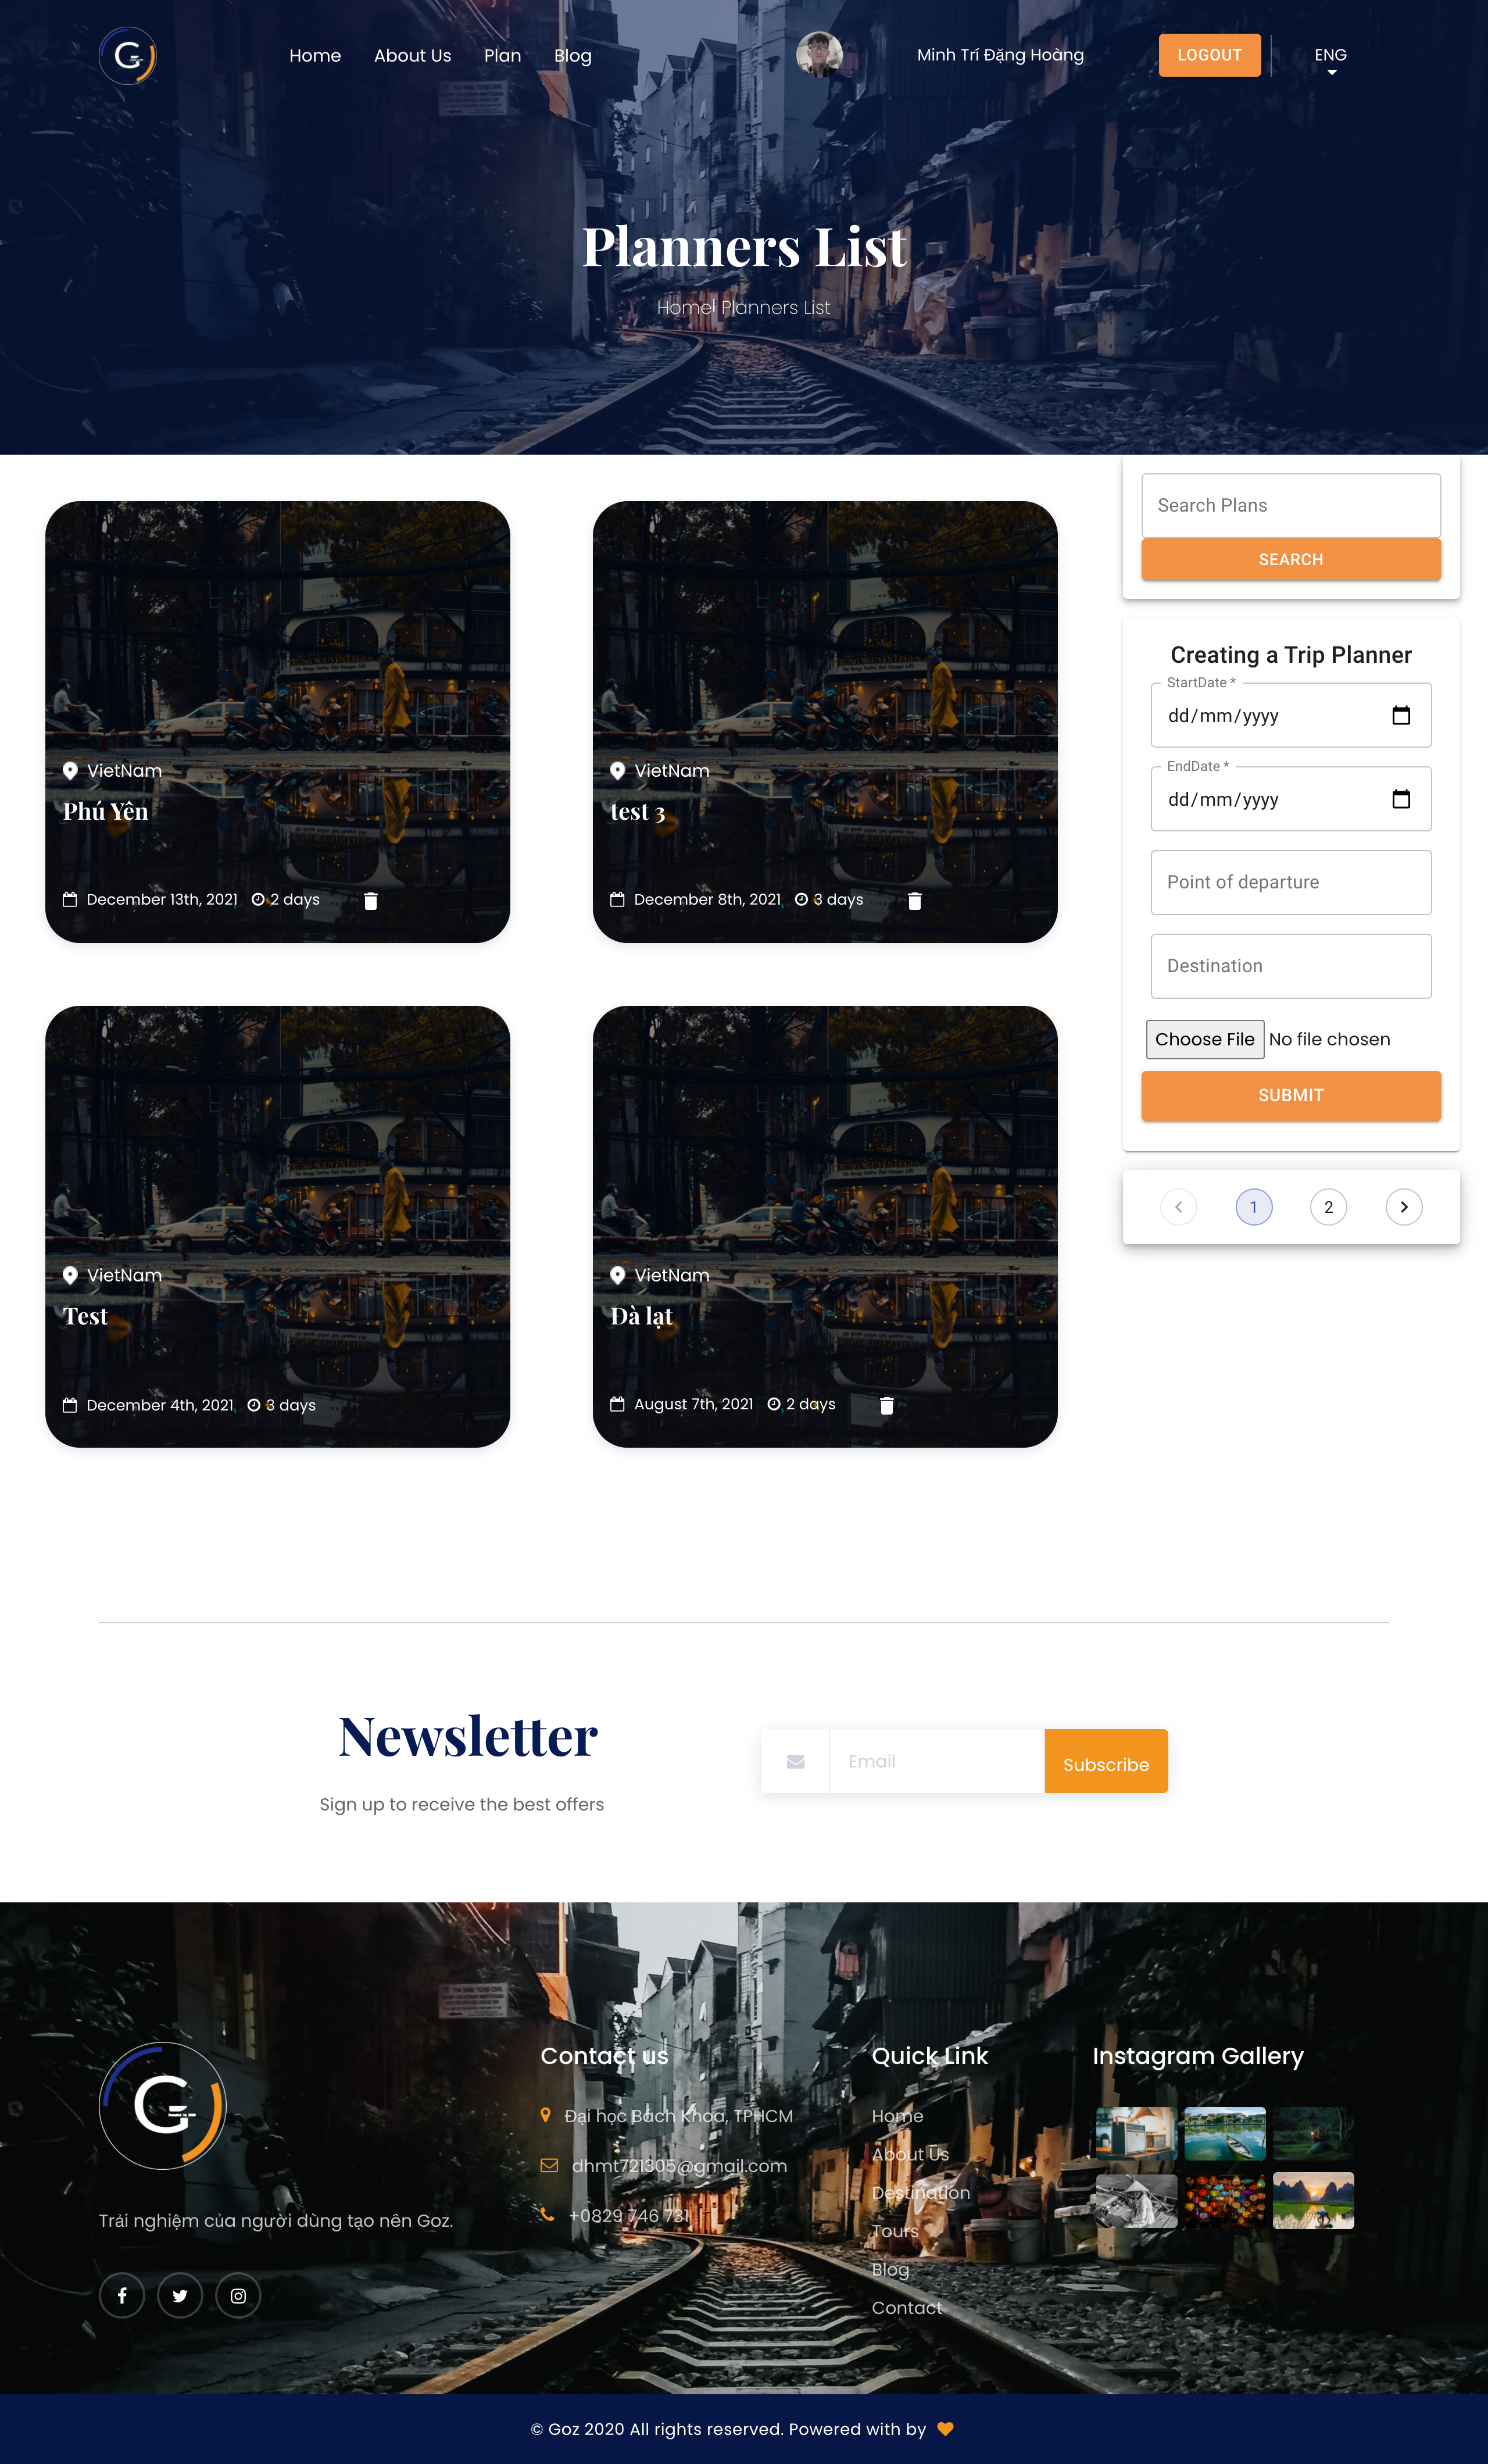
\includegraphics[width=15cm]{document/image/listplans.png}
    \captionof{figure}{Danh sách kế hoạch}
\end{center}

\begin{center}
    \captionsetup{type=figure}  
    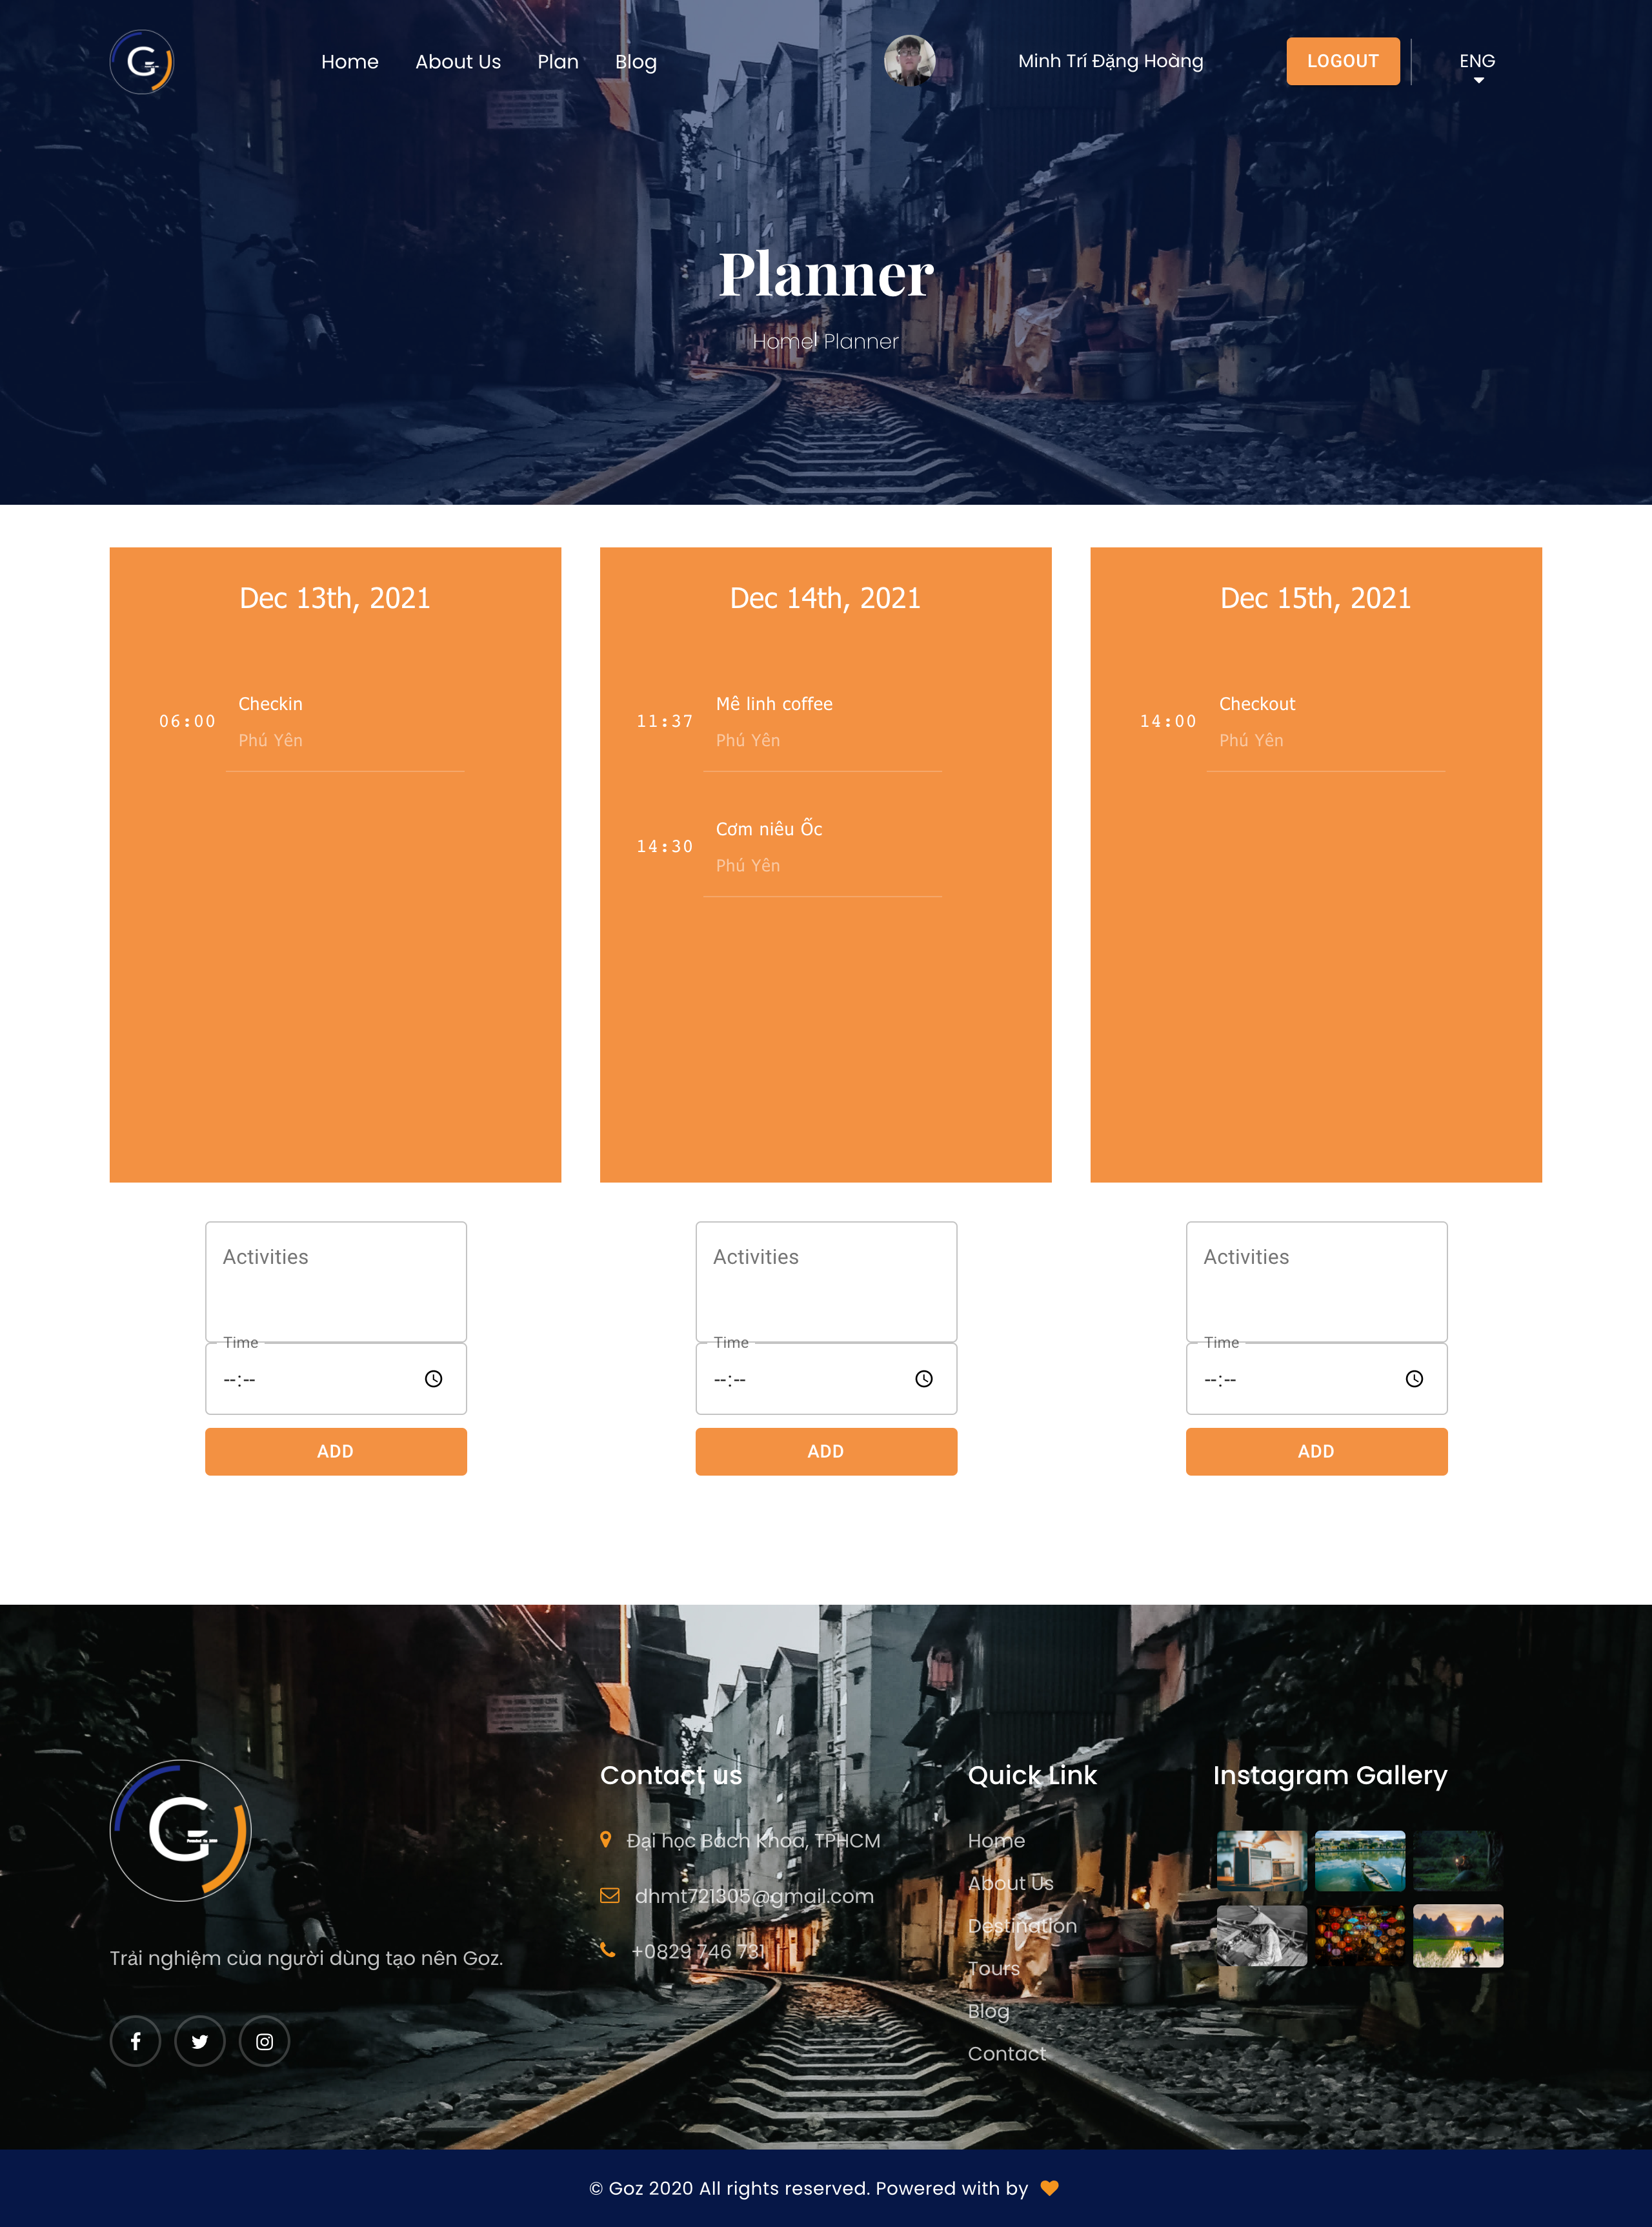
\includegraphics[width=15cm]{document/image/plan.png}
    \captionof{figure}{Plan}
\end{center}
\clearpage
\begin{center}
    \captionsetup{type=figure}  
    \includegraphics[width=15cm]{document/image/addhoatdong.png}
    \captionof{figure}{Plan thêm hoạt động cho kế hoạch}
\end{center}

\clearpage
\section{Triển khai dự án thực tế}
\subsection{Tìm hiểu heroku}
\begin{center}
    \captionsetup{type=figure}  
    \includegraphics[width=15cm]{document/image/heroku.png}
    \captionof{figure}{Heroku}
\end{center}

Heroku là một nền tảng đám mây để xây dựng và triển khai ứng dụng. Cung cấp một cách đơn giản cho các nhà phát triển có thể tập trung vào việc phát triển sản phẩm mà không cần quan tâm hay có hiểu biết quá tường tận về máy chủ và phần cứng.
Heroku chạy các ứng dụng trong dynos, có hỗ trợ gói miễn phí và các addons hỗ trợ rất hữu ích. Heroku hỗ trợ nhiều ngôn ngữ lập trình như:

\begin{itemize}
    \item \textbf{Nodejs}
    \item Ruby
    \item Python
    \item PHP
    \item Java
    \item ...
\end{itemize}
Thêm vào đó, Heroku còn hỗ trợ SSL miễn phí, cung cấp database, hỗ trợ làm việc theo team và cung cấp liên kết với Git hiệu quả và đơn giản.

\subsection{Triển khai dự án lên Heroku}
Với mong muốn đưa vào thử nghiệm thực tế, dự án đã được deploy lên Heroku theo đường dẫn sau: 
\href{https://travelgoz.com/vi/}{Du lịch Goz}







% Người dùng sử dụng tài khoản trường Đại học Bách Khoa của mình để đăng nhập. Sau khi đăng nhập thành công, hệ thống xác thực tập trung (SSO) sẽ trả về cho hệ thống email tài khoản của người dùng. Lúc này hệ thống sẽ kiểm tra, email nhận được đã được quản trị viên thêm vào hệ thống thì người dùng sẽ đăng nhập được vào hệ thống và thực hiện các chức năng với vai trò của mình.\\

% Đối với từng vai trò, sau khi đăng nhập vào hệ thống sẽ có các menu như sau:
% \begin{center}
%   \captionsetup{type=figure}
%   \includegraphics[width=15cm]{image/canbo.png}
%   \captionof{figure}{Menu của người dùng là CBCNV của trường}
% \end{center}
% \begin{center}
%   \captionsetup{type=figure}
%   \includegraphics[width=15cm]{image/eventManager.png}
%   \captionof{figure}{Menu của người dùng là quản lý sự kiện}
% \end{center}
% \begin{center}
%   \captionsetup{type=figure}
%   \includegraphics[width=15cm]{image/diemRenLuyenAdmin.png}
%   \captionof{figure}{Menu tất cả các vai trò về điểm rèn luyện}
% \end{center}
% \clearpage
% \section{Các trang tính năng quản lý cụ thể}
% \subsection{Quản lý bài viết sự kiện} \label{news_management}
% \subsubsection{Quản lý danh mục} \label{category_management}
% Quản trị viên có thể \textbf{thêm, sửa, xoá, thay đổi thứ tự} các danh mục thuộc loại sự kiện. Các danh mục này sẽ được dùng trong phần \textbf{tạo/chỉnh sửa} một sự kiện cụ thể (hình \ref{fig:category_news}).
% \begin{figure}[H]
%     \centering
%     \begin{subfigure}[b]{0.6\linewidth}
%         \includegraphics[width=\linewidth]{image/danh_sach_category.png}
%         \caption{Danh sách danh mục của sự kiện}
%     \end{subfigure}
%     \begin{subfigure}[b]{0.3\linewidth}
%         \includegraphics[width=\linewidth]{image/chinh_sua_category.png}
%         \caption{Chọn tên thành phần}
%     \end{subfigure}
%     \caption{Cấu hình danh mục cho sự kiện}
%     \label{fig:category_news}
% \end{figure}
% \subsubsection{Chỉnh sửa sự kiện}
% Quản trị viên có thể \textbf{tạo mới, chỉnh sửa, xoá} sự kiện. Hình \ref{fig:chinh_sua_news} trình bày giao diện chỉnh sửa sự kiện 
% về \textbf{tiêu đề, kích hoạt, hình ảnh, ngày tháng} của sự kiện. Quản trị viên cũng có thể \textbf{gán các danh mục} cho sự kiện đang chỉnh sửa,
% các danh mục này có được từ việc tạo danh mục sự kiện ở phần \ref{category_management} (hình \ref{fig:gan_danh_muc}).

% \begin{figure}[H]
%     \centering
%     \includegraphics[width=\linewidth]{image/chinh_sua_news.png}
%     \caption{Chỉnh sửa sự kiện: tiêu đề, hình ảnh, thời gian}
%     \label{fig:chinh_sua_news}
% \end{figure}

% \begin{figure}[H]
%     \centering
%     \includegraphics[width=7cm]{image/gan_danh_muc.png}
%     \caption{Gán danh mục cho sự kiện}
%     \label{fig:gan_danh_muc}
% \end{figure}
% \begin{figure}[H]
%     \centering
%     \includegraphics[width=12cm]{image/tom_tat_tin_tuc.png}
%     \caption{Tóm tắt, nội dung của sự kiện}
%     \label{fig:tom_tat_tin_tuc}
% \end{figure}


% Ngoài ra, quản trị viên cũng có thể chỉnh sửa phần \textbf{tóm tắt} cũng như là \textbf{soạn thảo nội dung} của sự kiện (hình \ref{fig:tom_tat_tin_tuc})

% \subsection{Quản lý sự kiện}
% \subsubsection{Năm học xét điểm rèn luyện, người đại diện, số lượng đăng ký, điểm rèn luyện, công tác xã hội, câu hỏi sự kiện}
% \begin{figure}[H]
%  \centering
%     \includegraphics[width=16cm]{image/chinh_sua_event_2.png}
%     \caption{Cấu hình cho sự kiện}
%     \centering
%     \label{fig:chinh_sua_event}
% \end{figure}
% \begin{figure}[H]
%     \centering
%     \includegraphics[width=13cm]{image/cau_hoi_su_kien.png}
%     \caption{Thiết lập câu hỏi cho sự kiện}
%     \label{fig:cau_hoi_su_kien}
% \end{figure}
% Ở phần này, quản trị viên có thể chỉnh sửa một số tính năng khác của sự kiện như:
% \begin{itemize}
%     \item \textbf{Chương trình năm học:} Nếu sự kiện này thuộc một trong các chương trình của năm học nào đó, thì quản trị viên sẽ gán sự kiện đó với
%     chương trình năm học tương ứng. Việc gán sự kiện cho chương trình năm học sẽ giúp cho quản trị viên cũng như hệ thống thực hiện việc \textbf{chấm/quản lý
%     điểm rèn luyện} cho sinh viên.
%     \item \textbf{Tạo câu hỏi cho sự kiện:} sự kiện sẽ có phần đăng ký tham gia sự kiện cho sinh viên, nên công việc tạo form đăng ký là cần thiết. 
%     Mô tả ở hình \ref{fig:cau_hoi_su_kien} sẽ hỗ trợ quản trị viên trong công việc này và kết quả của form được trình bày như hình \ref{fig:home_dang_ky_su_kien}.
%     \begin{figure}[H]
%         \centering
%         \includegraphics[width=10cm]{image/home_dang_ky_su_kien.png}
%         \caption{Giao diện form đăng ký}
%         \label{fig:home_dang_ky_su_kien}
%     \end{figure}
% \end{itemize}
% \subsubsection{Danh sách sinh viên tham gia sự kiện}
% \begin{itemize}
%     \item Quản trị viên cũng có thể xem thông tin câu trả lời của sinh viên tham gia, và có thể xuất ra file excel danh sách tất cả sinh viên kèm theo câu trả lời của từng người (hình \ref{fig:xem_form_chi_tiet}).
%     \begin{figure}[H]
%         \centering
%         \includegraphics[width=15cm]{image/xem_form_chi_tiet.png}
%         \caption{Chi tiết câu trả lời}
%         \label{fig:xem_form_chi_tiet}
%     \end{figure}
%      \item Quản trị viên cũng có thể thêm sinh viên tham gia.
%     \begin{figure}[H]
%         \centering
%         \includegraphics[width=15cm]{image/add_student_join.png}
%         \caption{Thêm sinh viên tham gia}
%         \label{fig:add_student_join}
%     \end{figure}
%     \item Trong những sự kiện quan trọng (ví dụ như là sự kiện "Buổi định hướng phân ngành CSE - 2019") thì sẽ có số lượng sinh viên bắt buộc 
%     tham gia nhất định, trong trường hợp này quản trị viên có thể import danh sách sinh viên tham gia sự kiện thông qua file excel. Sau khi 
%     import thành công, hệ thống sẽ tự động gửi email/thông báo đến từng sinh viên về sự kiện đó (hình \ref{fig:import_ds_sinh_vien}).
%     \begin{figure}[H]
%         \centering
%         \includegraphics[width=10cm]{image/import_ds_sinh_vien.png}
%         \caption{Import danh sách sinh viên}
%         \label{fig:import_ds_sinh_vien}
%     \end{figure}
%     \clearpage
%     \item Quản trị viên cũng có thể điểm danh sinh viên (theo MSSV hoặc tên của sinh viên) tham gia sự kiện (hình \ref{fig:admin_diem_danh}). và xuất danh sách sinh viên bằng excel.
%     \begin{figure}[H]
%         \centering
%         \includegraphics[width=15cm]{image/admin_diem_danh.png}
%         \caption{Điểm danh sinh viên tham dự}
%         \label{fig:admin_diem_danh}
%     \end{figure}
%       \item Quản trị viên có thể xem được  viên (theo MSSV hoặc tên của sinh viên) tham gia sự kiện (hình \ref{fig:admin_diem_danh}). và xuất danh sách sinh viên bằng excel.
%     \begin{figure}[H]
%         \centering
%         \includegraphics[width=15cm]{image/danh_sach_sv_register.png}
%         \caption{Danh sách sinh sinh viên tham dự}
%         \label{fig:danh_sach_sv_register}
%     \end{figure}
% \end{itemize}
% \clearpage
% \subsection{Quản lý bộ tiêu chí}
% Trường Đại học Bách Khoa sẽ có đưa ra một bộ tiêu chí dùng để xét điểm rèn luyện của sinh viên cho cả năm học(theo Thông tư số 16 năm 2015 của Bộ GDĐT). Gồm các tiêu chí và yếu tố rèn luyện với các số điểm cộng trừ cụ thể và giới hạn số lần trong một học kỳ. Mỗi tiêu chí có thể được cộng và trừ nhiều điểm nhưng không được vuợt khung từng tiêu chí và ĐRL không quá 100. 
%  \begin{figure}[H]
%         \centering
%         \includegraphics[width=\linewidth]{image/bo_tieu_chi_chuan.png}
%         \caption{Bộ tiêu chí chuẩn của Trường Đại Học Bách Khoa}
%         \label{fig:bo_tieu_chi_chuan}
%     \end{figure}
%  Có thể chỉnh sửa, thêm mới, kích hoạt hoặc xoá các tiêu chí rèn luyện. Ngoài ra có thể thêm một yếu tố rèn luyện vào một tiêu chí. 
%  \begin{figure}[H]
%         \centering
%         \includegraphics[width=13cm]{image/thao_tac_tieu_chi.png}
%         \caption{Các thao tác với một tiêu chí rèn luyện}
%         \label{fig:thao_tac_bo_tieu_chi}
%     \end{figure}
% \begin{figure}[H]
%     \centering
%     \begin{subfigure}[b]{0.5\linewidth}
%         \includegraphics[width=\linewidth]{image/chinh_sua_tieu_chi.png}
%         \caption{Chỉnh sửa một tiêu chí rèn luyện}
%     \end{subfigure}
%     \begin{subfigure}[b]{0.5\linewidth}
%         \includegraphics[width=\linewidth]{image/add_yeu_to.png}
%         \caption{Thêm hoặc bớt các yếu tố}
%     \end{subfigure}
%     \caption{Chỉnh sửa một tiêu chí rèn luyện cụ thể}
% \end{figure}

% Chỉnh sửa, kích hoạt hoặc xoá các yếu tố rèn luyện. 
% \begin{figure}[H]
%     \centering
%     \begin{subfigure}[b]{0.5\linewidth}
%         \includegraphics[width=\linewidth]{image/thao_tac_yeu_to.png}
%         \caption{Thao tác yếu tố rèn luyện}
%     \end{subfigure}
%     \begin{subfigure}[b]{0.5\linewidth}
%         \includegraphics[width=\linewidth]{image/chinh_sua_yeu_to.png}
%         \caption{Chỉnh sửa một yếu tố}
%     \end{subfigure}
%     \caption{Chỉnh sửa một yếu tố rèn luyện cụ thể}
% \end{figure}
% \clearpage
% Các khoa sẽ có quyền được tạo bản sao từ bộ tiêu chí Trường hoặc các Khoa khác. Có thể chỉnh sửa lại sao cho phù hợp với Khoa đó.
% \begin{figure}[H]
%         \centering
%         \includegraphics[width=13cm]{image/clone_tieu_chi.png}
%         \caption{Tạo bản sao một bộ tiêu chí rèn luyện}
%         \label{fig:clone_tieu_chi}
% \end{figure}
% \begin{figure}[H]
%         \centering
%         \includegraphics[width=13cm]{image/bo_tieu_chi_cac_cap.png}
%         \caption{Bộ tiêu chí rèn luyện các cấp}
%         \label{fig:bo_tieu_chi_cac_cap}
% \end{figure}

 
% \subsection{Quản lý điểm rèn luyện}
% Hệ thống tổ chức quản lý điểm rèn luyện theo từng năm học. Quản trị viên có thể \textbf{theo dõi điểm rèn luyện} của tất cả sinh viên trong năm học đó.
% Những sinh viên có số điểm rèn luyện khác nhau sẽ hiển thị với những nền màu khác nhau. Ngoài ra, quản trị viên có thể xuất điểm rèn 
% luyện của năm học đó với tất cả sinh viên kèm các sự kiện mà sinh viên đã tham gia, quản trị viên còn có thể thực hiện thao tác \textbf{Cập 
% nhật lại điểm rèn luyện} nếu muốn (Chức năng này hệ thống đã lên lịch và cứ mỗi cuối tuần sẽ được tự động cập nhật lại).

% Ngoài ra mỗi cuối năm học sinh viên thực hiện chấm phiếu điểm rèn luyện. Phiếu chấm điểm rèn luyện được dựa trên những yếu tố rèn luyện(đi kèm minh chứng) dựa trên bộ tiêu chí rèn luyện chuẩn của \textbf{Trường Đại Học Bách Khoa}. Sau khi chấm sinh viên được thành phần ban cán sự lớp thực hiện việc duyệt/từ chối những yếu tố mà sinh viên chấm dựa trên những minh chứng có hợp lý hay không. Tương tự sau khi được ban cán sự lớp thông qua sẽ được giáo viên chủ nhiệm duyệt lại một lần nữa trước khi nộp về cho Khoa.

% Khoa sẽ là nơi tổng hợp điểm rèn luyện sinh viên cuối cùng và tiếp nhận phản hồi của sinh viên trước khi gửi kết quả điểm rèn luyện năm học đó về Trường.
% \subsubsection{Cấu hình điểm rèn luyện}
% \begin{itemize}
%     \item Quản trị viên sẽ thực hiện việc cấu hình điểm rèn luyện các email cần thiết.(hình \ref{fig:setting_drl}).
%     \begin{figure}[H]
%         \centering
%         \includegraphics[width=15cm]{image/setting_drl.png}
%         \caption{Cấu hình điểm rèn luyện}
%         \label{fig:setting_drl}
%     \end{figure}

% \item Quản trị viên có thể tiếp nhận phản hồi từ phía sinh viên về tình hình điểm rèn luyện hiện tại của họ, quản trị viên xem xét phản hồi và chỉnh sửa lại điểm rèn luyện cho sinh viên đó nếu cần thiết.
% \clearpage
% \begin{figure}[H]
%     \centering
%     \includegraphics[width=10cm]{image/phan_hoi_drl.png}
%     \caption{Phản hồi điểm rèn luyện từ sinh viên}
%     \label{fig:phan_hoi_drl}
% \end{figure}
% \begin{figure}[H]
%     \centering
%     \includegraphics[width=10cm]{image/chitiet_phanhoi_drl.png}
%     \caption{Nội dung phản hồi điểm rèn luyện từ sinh viên}
%     \label{fig:chitiet_phanhoi_drl}
% \end{figure}
% \item Quản trị viên có thể thêm, xoá và chỉnh sửa các chức vụ ban cán sự lớp để phục vụ cho mục đích sắp xếp lớp trong một Khoa.
% \begin{figure}[H]
%     \centering
%     \includegraphics[width=15cm]{image/chuc_vu_cs.png}
%     \caption{Thao tác với chức vụ các sự lớp}
%     \label{fig:chuc_vu_cs}
% \end{figure}
% \end{itemize}
% \subsection{Vai trò duyệt điểm rèn luyện}
% Sau khi nộp phiếu chấm điểm rèn luyện cần qua hai lần duyệt để đảm bảo tính trung thực, chính xác. Đầu tiên sẽ được duyệt bởi ban cán sự lớp. Sau đó được duyệt bởi giáo viên chủ nhiệm trước khi gửi về Khoa.
% \subsubsection{Ban cán sự lớp}
% Ban cán sự lớp sẽ tổng hợp điểm của các thành viên trong lớp của mình. Gửi email yêu cầu thành viên nộp phiếu chấm rèn luyện(nếu chưa nộp). Khoá phiếu chấm nếu quá hạn mà sinh viên chưa nộp.
% \begin{figure}[H]
%     \centering
%     \includegraphics[width=\linewidth]{image/can_su_cham.png}
%     \caption{Giao diện ban cán sự lớp duyệt điểm rèn luyện}
%     \label{fig:can_su_cham}
% \end{figure}
% Chi tiết từng sinh viên. Cán sự có thể chấm lại: thêm, chỉnh sửa yếu tố rèn luyện và để lại phản hồi.
% \begin{figure}[H]
%     \centering
%     \includegraphics[width=\linewidth]{image/detail_sv_cultivation.png}
%     \caption{Chi tiết duyệt phiếu chấm điểm rèn luyện}
%     \label{fig:detail_sv_cultivation}
% \end{figure}
% \begin{figure}[H]
%     \centering
%     \begin{subfigure}[b]{0.5\linewidth}
%         \includegraphics[width=\linewidth]{image/view_minh_chung.png}
%         \caption{Xem minh chứng của một yếu tố}
%     \end{subfigure}
%     \begin{subfigure}[b]{0.5\linewidth}
%         \includegraphics[width=\linewidth]{image/change_diem.png}
%         \caption{Chỉnh sửa điểm và để lại phản hồi}
%     \end{subfigure}
%     \caption{Duyệt phiếu chấm điểm rèn luyện sinh viên}
% \end{figure}
% \subsubsection{Giáo viên chủ nhiệm}

% Giáo viên chủ nhiệm lớp cũng sẽ có vai trò tương tự ban cán sự lớp có thể duyệt và phản hồi điểm rèn luyện sinh viên. Gửi email yêu cầu thành viên nộp phiếu chấm rèn luyện(nếu chưa nộp). Khoá phiếu chấm nếu quá hạn mà sinh viên chưa nộp.

% Ngoài ra còn có thể gán thành phần ban cán sự lớp cho lớp mình chủ nhiệm tại mỗi năm học.
% \begin{figure}[H]
%     \centering
%     \includegraphics[width=\linewidth]{image/gvcn_assign_student.png}
%     \caption{Giao diện gán thành phần ban cán sự cho lớp chủ nhiệm}
%     \label{fig:gvcn_assign_student}
% \end{figure}
% \subsubsection{Trợ lý sinh viên}

% Trợ lý sinh viên sẽ có vai trò sắp xếp giáo viên chủ nhiệm cho Khoa mỗi năm học. Có thể gán luôn cả thành phần ban cán sự lớp.

% \begin{figure}[H]
%     \centering
%     \includegraphics[width=\linewidth]{image/list_gvcn.png}
%     \caption{Danh sách giáo viên chủ nhiệm theo từng năm học}
%     \label{fig:list_gvcn}
% \end{figure}

% \begin{figure}[H]
%     \centering
%     \includegraphics[width=\linewidth]{image/create_gvcn.png}
%     \caption{Tạo giáo viên chủ nhiệm theo từng năm học}
%     \label{fig:create_gvcn}
% \end{figure}
% Ngoài ra còn quản lý điểm rèn luyện cho sinh viên cả Khoa. Duyệt điểm rèn luyện sinh viên các năm học. Có thể chỉnh sửa cả điểm chấm của cán sự lớp và giáo chủ nhiệm nếu như không hợp lý.
% \begin{figure}[H]
%     \centering
%     \includegraphics[width=\linewidth]{image/class_drl.png}
%     \caption{Quản lý điểm rèn luyện các lớp của Khoa}
%     \label{fig:class_drl}
% \end{figure}
% \clearpage
% Chi tiết giao diện từng lớp và từng sinh viên trong vai trò trợ lý sinh viên. Trợ lý sinh viên có thể thấy được điểm rèn luyện mà sinh viên, cán sự lớp và giáo viên chủ nhiệm chấm.
% \begin{figure}[H]
%     \centering
%     \includegraphics[width=\linewidth]{image/class_detail_drl.png}
%     \caption{Giao diện chi tiết một lớp trong Khoa}
%     \label{fig:class_detail_drl}
% \end{figure}
% \begin{figure}[H]
%     \centering
%     \includegraphics[width=\linewidth]{image/student_detail_drl.png}
%     \caption{Giao diện chi tiết một sinh viên trong lớp}
%     \label{fig:student_detail_drl}
% \end{figure}
% \clearpage
% Trợ lý sinh viên chỉnh sửa được điểm rèn luyện cán sự lớp chấm, giáo viên chủ nhiệm chấm và để lại phản hồi.
% \begin{figure}[H]
%     \centering
%     \includegraphics[width=13cm]{image/student_fix_drl.png}
%     \caption{Chỉnh sửa điểm một sinh viên trong lớp}
%     \label{fig:student_fix_drl}
% \end{figure}
% Dữ liệu hiện tại không đồng nhất với dữ liệu phòng đào tạo nên trợ lý sinh viên có quyền chỉnh sửa lớp của sinh viên để đúng với thực tế.
% \begin{figure}[H]
%     \centering
%     \includegraphics[width=\linewidth]{image/troly_class.png}
%     \caption{Danh sách lớp trong Khoa đi kèm với sĩ số}
%     \label{fig:troly_class}
% \end{figure}
% \clearpage
% Chi tiết giao diện một lớp và chỉnh sửa một lớp học cho sinh viên.
% \begin{figure}[H]
%     \centering
%     \includegraphics[width=13cm]{image/troly_class_fix.png}
%     \caption{Chỉnh sửa lớp cho một sinh viên}
%     \label{fig:troly_class_fix}
% \end{figure}
% Ngoài ra trợ lý sinh viên còn có thể ghi đè dữ liệu sinh viên bằng cách upload file excel của lớp cần chỉnh sửa dữ liệu.
% \begin{figure}[H]
%     \centering
%     \includegraphics[width=\linewidth]{image/troly_class_upload.png}
%     \caption{Upload file excel danh sách lớp dữ liệu sinh viên}
%     \label{fig:troly_class_upload}
% \end{figure}
% \begin{figure}[H]
%     \centering
%     \begin{subfigure}[b]{0.8\linewidth}
%         \includegraphics[width=\linewidth]{image/troly_list_upload.png}
%         \caption{Upload file excel danh sách lớp cần chỉnh sửa dữ liệu}
%     \end{subfigure}
%     \begin{subfigure}[b]{0.8\linewidth}
%         \includegraphics[width=\linewidth]{image/troly_confirm_upload.png}
%         \caption{Xác nhận ghi đè dữ liệu}
%     \end{subfigure}
%     \caption{Upload dữ liệu lớp học của sinh viên}
% \end{figure}
% \section{Sinh viên}
% Sinh viên có thể theo dõi tình hình điểm rèn luyện của mình theo từng năm học, chi tiết bao gồm danh sách các hoạt động đã tham gia trong năm học kèm
% điểm rèn luyện đạt được và tổng điểm rèn luyện hiện tại mà sinh viên đó đã tích luỹ (hình \ref{fig:student_cultivation}).
% \begin{figure}[H]
%     \centering
%     \includegraphics[width=\linewidth]{image/student_cultivation.png}
%     \caption{Điểm rèn luyện của sinh viên theo năm học}
%     \label{fig:student_cultivation}
% \end{figure}
% Sinh viên sẽ thực hiện chấm phiếu chấm điểm rèn luyện mỗi cuối năm học. Bộ tiêu chí dựa trên bộ tiêu chí chuẩn của nhà Trường và được tuỳ chỉnh phù hợp cho mỗi Khoa. Mỗi yếu tố sẽ có điểm cộng/trừ tương ứng. Sinh viên cần nộp kèm minh chứng để xác minh cho yếu tố để được duyệt.(hình \ref{fig:student_cultivation_page}).
% \begin{figure}[H]
%     \centering
%     \includegraphics[width=\linewidth]{image/student_cultivation_page.png}
%     \caption{Chi tiết phiếu chấm điểm rèn luyện mỗi năm học}
%     \label{fig:student_cultivation_page}
% \end{figure}
